\chapter{Implementation}\label{C:implementation}
The Bayesian estimator proposed in this report has required comprehensive technical implementation to provide a strong comparative analysis of its effectiveness. These components include:

\begin{itemize}
    \item implementation of techniques proposed by previous studies for this problem domain,
    \item the validation of the implementation of those competing techniques such that each of their distinct features can be accurately compared and analysed,
    \item creation of the proposed estimator with consideration for its special input requirements compared to the previous techniques, and
    \item a fair test procedure and algorithm to compare and contrast the different estimators.
\end{itemize}

These several components were developed, prototyped, and analysed in \textit{MATLAB}. This is such that the analysis may be general. Therefore, the results from here can be transferred towards other platforms such as an embedded implementation.



\section{Existing Techniques}
The existing techniques were implemented and validated against the published results. This allows for analysis beyond the specific case study density functions discussed within their respective publications. This means that we may obtain a valid comparison of methods via a larger variety of representative data. In addition, there is no known publicly published implementation of the techniques by the authors, hindering implementation.

\subsection{Validation of Implementation}
The validation framework compares an extraction of the original estimate with the reproduced estimate. This allows for an accurate perspective of any analysis made between the benchmark estimators and the proposed estimator. Figure \ref{fig:validate_recreated_models} demonstrates the validation topology used by this project.

\begin{figure}[h]
    \centering
    \includegraphics[width=\textwidth]{implementation/ValidateRecreatedModels.pdf}
    \caption{Test architecture for recreating the existing estimators in the literature}
    \label{fig:validate_recreated_models}
\end{figure}

The components of the validation framework process are as follows:

\begin{enumerate}
    \item The image extractor uses an image of the model in the publication to acquire the published density function and its technique's estimate. An off the shelf image extractor was used \cite{webplotdigitizer}.
    \item The interpolator discussed in Section \ref{section:oneDimInterpolation} is used so we may have direct compatibility and comparability between the different frameworks
    \item The estimator being validated develops its estimate of the density function
    \item The comparison component allows for analysis of the deviations between the true estimate and the recreated estimate. This takes the form of visual display and the numerical indicators of error and deviation.
\end{enumerate}

We use the published model density functions analysed by Gruber et al. \cite{GruberT2Estimation2013} for the validation of the different recreations of the techniques. This means that any analysis we make on technique accuracy here may be representative of actual data. Figure \ref{fig:T2_validation_models} illustrates each of the models used for system validation.

\begin{figure}[htb!]
    \centering
    \begin{subfigure}[b]{0.49\textwidth}
        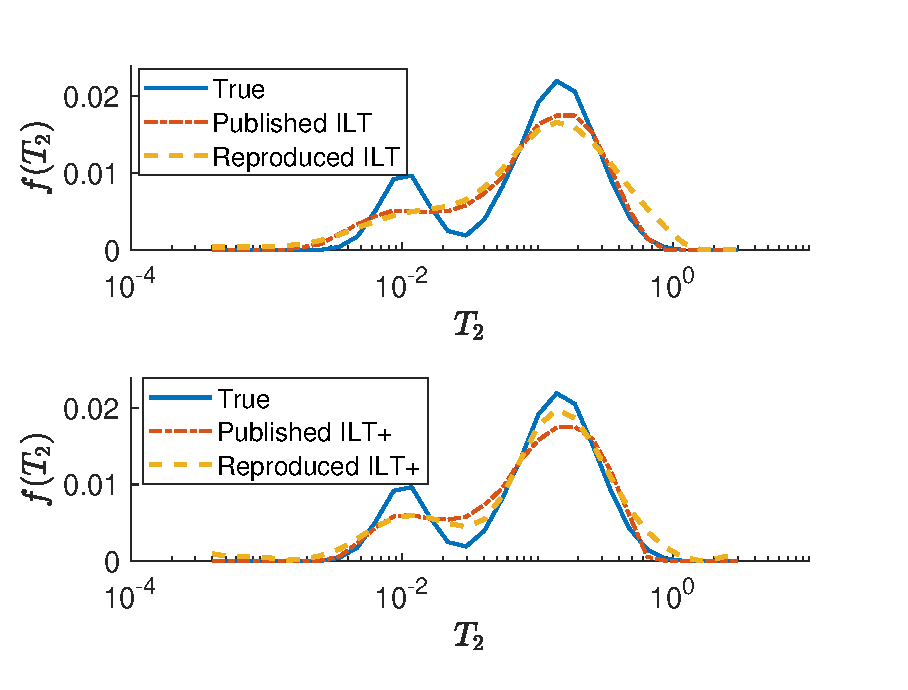
\includegraphics[width=\textwidth]{implementation/model1.eps}
        \subcaption{Model \#1}
        \label{fig:model1True}
    \end{subfigure}
    \begin{subfigure}[b]{0.49\textwidth}
        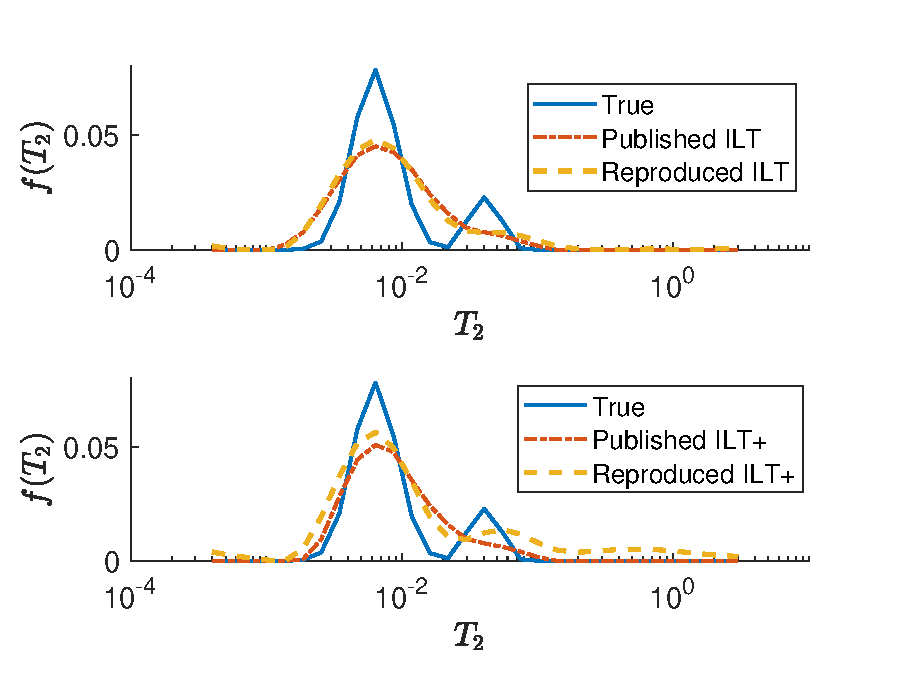
\includegraphics[width=\textwidth]{implementation/model2.eps}
        \subcaption{Model \#2}
        \label{fig:model2True}
    \end{subfigure}
    \begin{subfigure}[b]{0.49\textwidth}
        \includegraphics[width=\textwidth]{implementation/model3.eps}
        \subcaption{Model \#3}
        \label{fig:model3True}
    \end{subfigure}
    \begin{subfigure}[b]{0.49\textwidth}
        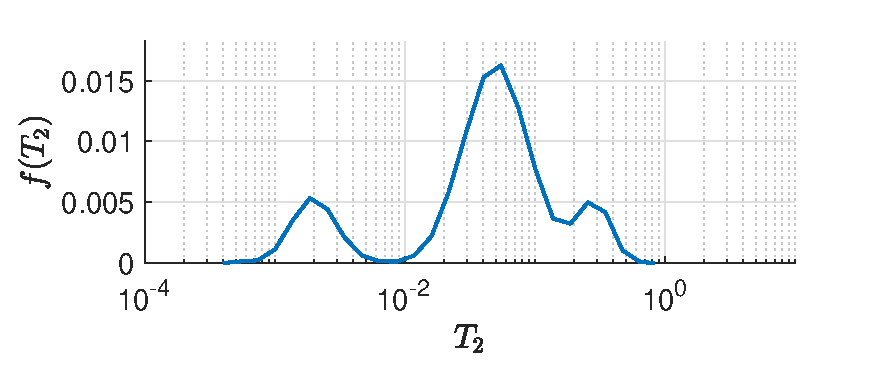
\includegraphics[width=\textwidth]{implementation/model4.eps}
        \subcaption{Model \#4}
        \label{fig:model4True}
    \end{subfigure}    
    \caption{The $T_2$ density functions of the models used for system validation}
    \label{fig:T2_validation_models}
\end{figure}


\subsection{Inverse Laplace Transform Approximation (ILT)} \label{section:ILTImplementation}
The canonical benchmark for density function estimation is the ILT approximation detailed in \cite{Venk2DFredholm2002} and Section \ref{section:ILT}. This project explores one-dimensional density functions rather than the two dimensional kind detailed by Venkataramanan et al. \cite{Venk2DFredholm2002}. This meant that the re-implementation tended towards the one-dimensional case proposed by the Butler-Reeds-Dawson method instead \cite{BulterReedsDawsonMethod1981}.




\subsubsection{Non-uniform SNR}
The simulation implementation from Gruber et al. \cite{GruberT2Estimation2013} is complicated by the inclusion of additional short pulse sequences that accompany the typical long pulse sequence. There are a series of thirty pulses repeated 10 times that increase the SNR for short relaxation times. This means that to reproduce the technique exactly, this component had to be reproduced as well. The method of implementation is as follows:

\begin{enumerate}
    \item Simulate the data for only 30 samples in the time domain 10 times (short pulses)
    \item Average these 10 pulse sequence results together
    \item Replace the first 30 values of the long sequence with the new averaged short pulse sequence results
    \item Scale the first 30 rows of the kernel matrix, $K$, by the SNR increase given by the short pulse sequence. We do the same for the measurement vector.
\end{enumerate}

\begin{figure}
    \centering
    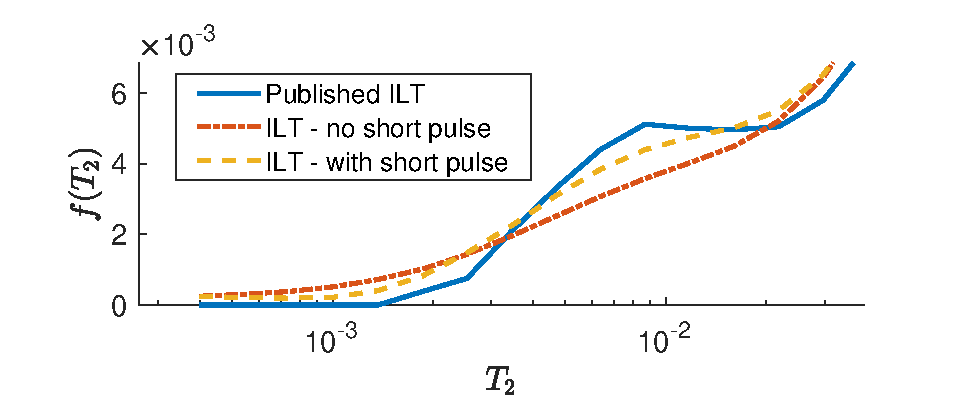
\includegraphics[width = 0.9\textwidth]{implementation/recreate_short_pulse.eps}
    \caption{Recreation of model 1 (Fig. \ref{fig:model1True}) ILT from Gruber et al. \cite{GruberT2Estimation2013} with and without the inclusion of repeated short pulse sequences.}
    \label{fig:non_uniform_SNR}
\end{figure}
 Figure \ref{fig:non_uniform_SNR} demonstrates the effect of accounting for a short pulse sequence in estimator recreation. As we can see, the reproduced technique's estimate is more sensitive for short relaxation. This in turn corresponds to a closer reproduction to the published result. Therefore, this methodology provides a more accurate representation of short relaxation times for our reproduction of the ILT experimental results in \cite{GruberT2Estimation2013}.




\subsubsection{Scaling the Noise}
The published noise standard deviation of 0.1 and an SNR of 10  in \cite{GruberT2Estimation2013} requires that the signal power be unity. However, the density functions benchmarked in the publication do not have unity power, i.e, the power of the measured signal before noise is added is not unity ($P_{\text{signal}} = \frac{1}{N_2}\sum^{N_2}_1 (m_i)^2 \neq 1$). Therefore, the noise standard deviation is scaled to achieve the published SNR such that the results can be recreated.

\subsubsection{$T_2$ Axis}
The $T_2$ axis of the density function estimate is a crucial aspect to reproduce due to the high variability that may come from an ill-conditioned problem.
The time axis was assumed to be defined for times from $2\times t_\text{sample}$ to 3 seconds as the simulation results in \cite{GruberT2Estimation2013} are bounded within these values. The $2\times t_\text{sample}$ bound is justified by the Shannon Sampling theorem \cite{shannon1949communication}. A sample period of $t_\text{sample}$ may only fully reconstruct T2 relaxation times of more than $2\times t_\text{sample}$ . In addition, the attention to this specific aspect of an inversion is justified by recent research into estimation sensitivity for that region of the $T_2$ domain \cite{venkataramanan2015newPorosity}.

\subsection{ILT+}
This technique requires a significant amount of complexity as it combines moment estimation by Venkataramanan et al. \cite{VenkMellin2010}, tapered area estimation by Gruber et al. \cite{GruberLinearFunctionals2013}, and the initial ILT methods by Venkataramanan et al. \cite{Venk2DFredholm2002} and Butler et al \cite{BulterReedsDawsonMethod1981}. The implementation follows many of the same points as the ILT method discussed in Section \ref{section:ILTImplementation}.

\begin{figure}[ht!]
    \centering
    \begin{subfigure}{1\textwidth}
        \centering
        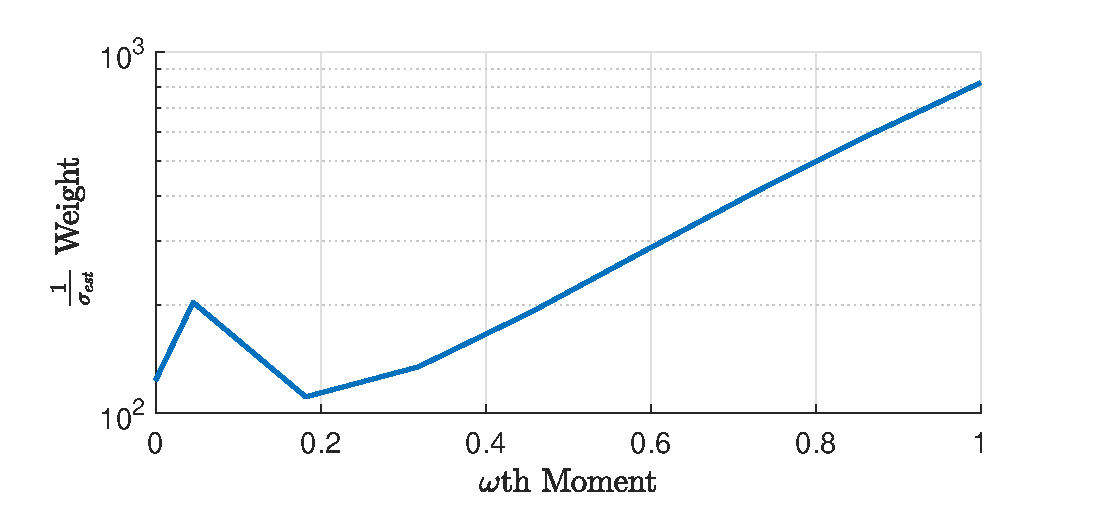
\includegraphics[width=0.8\textwidth]{implementation/moment_weighting.eps}
        \subcaption{Weighting of each moment estimation's certainty on a logarithmic scale}
    \label{fig:moment_estimator_weight}
    \end{subfigure}
    \begin{subfigure}{1\textwidth}
        \centering
        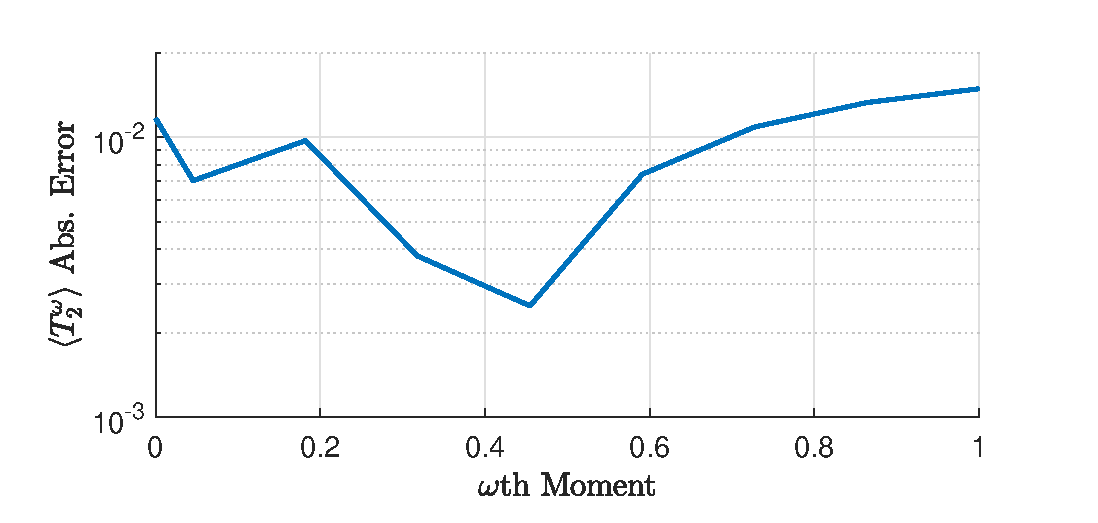
\includegraphics[width=0.8\textwidth]{implementation/moment_abs_error.eps}
        \subcaption{Absolute error of the moment estimation on a logarithmic scale}
        \label{fig:moment_estimator_abs_err}
    \end{subfigure}
    \caption{A comparison of the certainty alongside the absolute error of the reproduced moment estimate for SNR = 10.}
    \label{fig:problems_moment_est}
\end{figure}

\subsubsection{Moment Estimator} \label{section:moment_est_implementation}
The ILT+ implementation was adversely complicated by the inclusion of the moment estimator detailed in Section \ref{section:moment_estimation} and given by Venkataramanan et al \cite{VenkMellin2010}. One of the main problems with it was with robustness and error. In order to compensate for this, we modify its weighting so that we may at least acquire indicative results for the evaluation in Chapter \ref{C:evaluation}.




To demonstrate a problem encountered in implementing the moment estimator in the estimator framework, we examine the moment estimation for model 1 from Gruber et al \cite{GruberT2Estimation2013} (shown in Figure \ref{fig:model1True}). 



Figure \ref{fig:moment_estimator_weight} indicates that as higher moments are estimated, we have a higher weighting for that estimate. However, in Figure \ref{fig:moment_estimator_abs_err} we can see that the absolute error increases for where $\omega > 0.5$. This is problematic as the implementation weights these more erroneous points more highly, i.e. the optimisation framework is more certain about worse estimates.

Given this issue with the implemented moment estimator there is a need to diminish its dependence on worse estimates. This diverges from the published results. However, we still preserve indicative trends of performance for the comparative analysis.

\begin{figure}[htb!]
    \centering
    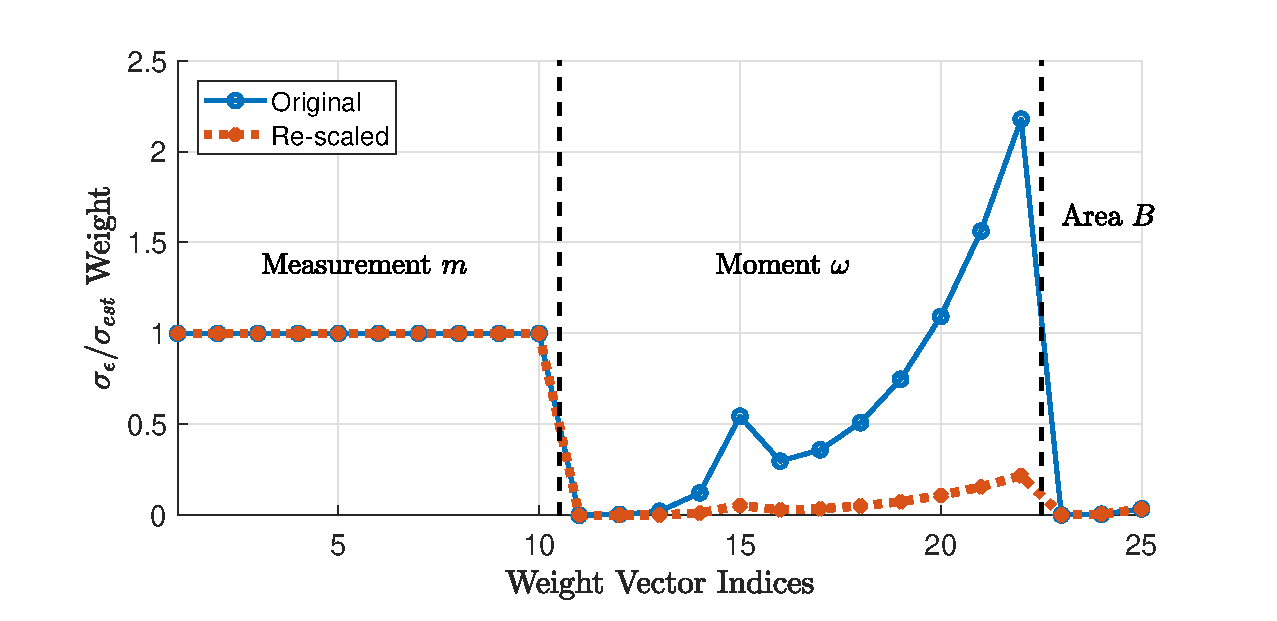
\includegraphics[width = 0.9\textwidth]{implementation/new_weighting_iltx.eps}
    \caption{Comparison of the original and altered weight vectors for ILT+ to allow for analysis of general indicative performance}
    \label{fig:diff_ILT+}
\end{figure}

Figure \ref{fig:diff_ILT+} demonstrates the augmented weighting regime for our implementation of ILT+. The moment weightings are reduced tenfold while all others remain the same so that the moment estimation may not overpower the overall estimation. This amount of reduction was done so that the implementation of the ILT+ would follow to an extent the published ILT+ results.





\iffalse
\subsubsection{Regularisation for ILT+}
The starting regularisation value used before the iterative process has a large effect on the resulting estimate for the ILT+ using the BRD method \cite{BulterReedsDawsonMethod1981}. For example, if the initial $\alpha$ were a very low number such as 0.1 to 1 (less than 10\% the published regularisation average), the result would require inversion of a poorly conditioned matrix. A large $\alpha$ on the other hand has a more stable start point. Figure \ref{fig:ilt+sensitivity} demonstrates the difference in an ILT+ estimate from choosing a different regularisation parameter with the same random seed. This aspect severely impacts implementation and make it difficult to reproduce the published results.

\begin{figure}
    \centering
    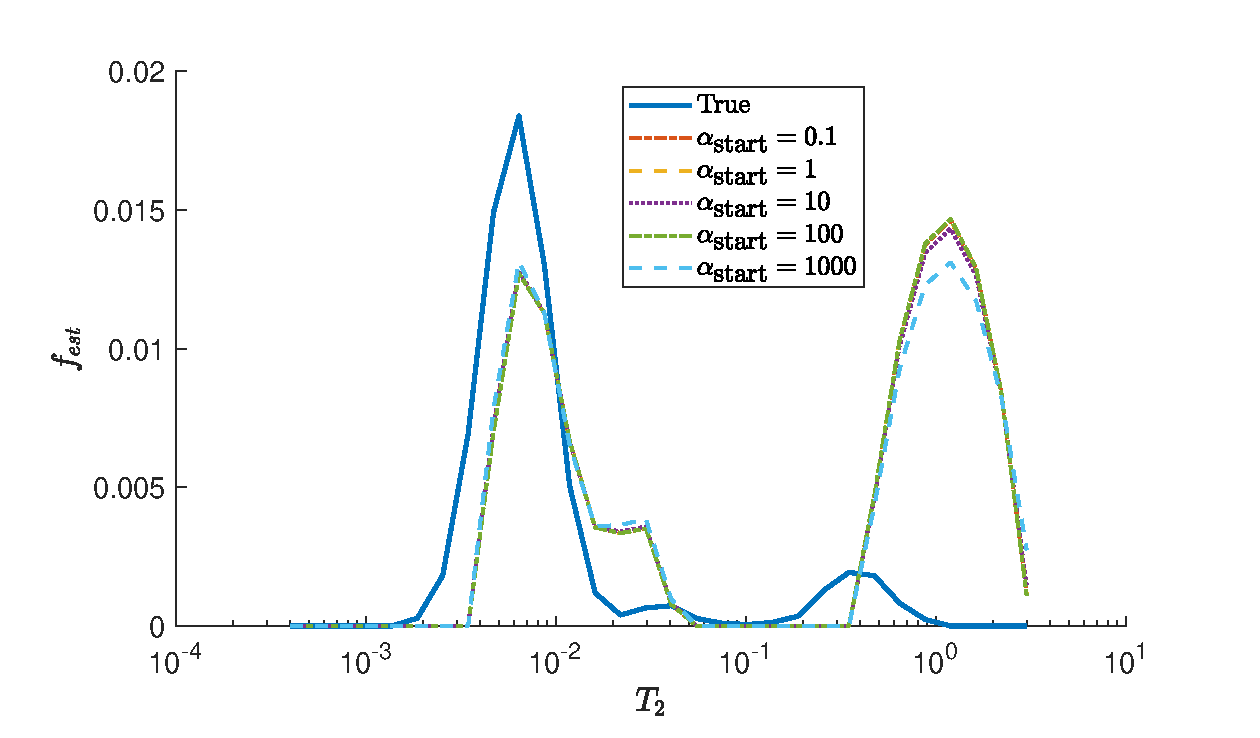
\includegraphics[width=\textwidth]{implementation/ILT+Regularisation.eps}
    \caption{Sensitivity to a start $\alpha$ in inversion for ILT+}
    \label{fig:ilt+sensitivity}
\end{figure}
\fi

\subsection{Tapered Area Estimator}
The tapered area estimator has a far simpler set up compared to the previous approximation techniques. This is due to it being fully self-contained and analytically tractable. It contains the exponential Haar transform detailed in \cite{GruberLinearFunctionals2013} and Section \ref{ss:taperedAreas}. It is a simple dot product between the time domain version of the transform and the measurement data per (\ref{eq:estTaperedAreas})

\section{Bayesian Technique}
The implementation of the Bayesian technique is more comparable to the tapered area estimator rather than the regularised least squares methods of the ILT and ILT+. This is due to the Gaussian assumption of the prior density function and the measurement data permitting an analytic approach to implement the estimator (as discussed in Section \ref{section:bayesTechniqueDesign}). The implementation is compared with the results obtained by Teal to allow for validation \cite{paulTeal_NMRBayes}.

\subsection{Estimator Architecture}
We adopt a computational sequence for the Bayesian technique to minimise unnecessary computation. The sequence, as shown also in Figure \ref{fig:bayesian_framework}, is as follows:
\begin{enumerate}
    \item we take the high quality known density functions and construct our prior mean and covariance before any time sensitive procedures. The prior can be constructed before estimation
    \item calculate the estimate density function, the mean of the Bayesian posterior, using (\ref{eq:posteriorProbability})
\end{enumerate}


The procedure requires no iterative computation like the ILT and ILT+, providing potential for less computation time. This is because the time consuming computation of the prior function does not have to be done within time-constrained use.






\section{Test Environment}
The test environment's implementation required attention so that it provided immediate comparability and fairness. The implementation of the test environment is required to be such that it provides an illuminating and fair comparison of the different techniques. The code for this can be found in \cite{dobbie_2018_test_Env}.


\subsection{Test Architecture}
The test architecture that compares each of estimators aims to demonstrate the uncertainty and typical performance of all of the techniques. In order to keep the Bayesian estimator from directly accessing the exact sample it is testing, leave one-out cross validation (as discussed in Section \ref{section:crossValidation}) is utilised for the evaluation process. Figure \ref{fig:test_architecture} details the architecture of the test setup. Table \ref{tab:test_variables} outlines the variables set for this test architecture. Any variation from these variables in the evaluation will be explicitly stated.


\begin{table}[h]
    \centering
    \begin{tabular}{l c l}
        \toprule
         & Variable  &     \hfill   Experimental Value \\
        \midrule
        $N_2$ & Number of Time Samples & 2500 \\
        $N_y$ & Number of Bins in T2 domain & 30 \\
        $t_E$ & Sample Period & \SI{200}{\micro\second}\\
        $T_2$ & Axis Bounds & \SI{400}{\micro\second} to 10 s \\
        $SNR_{\text{linear}}$ & Signal to Noise Ratio (Uniform) & 10 \\
        $T_c$ & Bound Fluid Cut-off & 33 ms \\
        \bottomrule
    \end{tabular}
    \caption{The variables used for the test architecture.}
    \label{tab:test_variables}
\end{table}



\begin{figure}[h]
    \centering
    \includegraphics[width=\textwidth]{implementation/test_arch2.pdf}
    \caption{The overall test setup to compare each of the estimators fairly.}
    \label{fig:test_architecture}
\end{figure}



An extension of the test architecture can allow for an analysis of how different cut-off times lead to different performance. This provides a perspective of when one technique may be more suitable than another technique. This comes at the cost of computational time, as estimating many samples over $N_y$ different cut off times for several techniques requires a non-trivial amount of computation. 


\subsection{Implementation Conclusions}

Throughout Chapter \ref{C:implementation}, there has been detailed analysis of the implementation of each of the estimators. Most of the complications came from quality issues in reproducing the existing techniques. The absence of published code by the authors made high quality reproduction non-trivial. However, the compromises made still allow for an indication of typical technique performance and trends. These aspects allow for the detailed evaluation in Chapter \ref{C:evaluation}.






\iffalse
In addition to the test environment, there is also a visual comparison of different case study density functions. There are published results by Gruber et al. \cite{GruberLinearFunctionals2013} that form a typical benchmark of the density functions that will be estimated. Even though some of the previously published results could not be reproduced exactly in the re-implemented estimators, the Bayesian technique can still be compared with definitive previous results.
\fi